\documentclass[aspectratio=169, 9pt]{beamer}

% Theme and color settings for dark theme
\usetheme{Madrid}
\usecolortheme{owl}
% Custom colors for dark theme
\definecolor{backgroundblack}{RGB}{15,15,15}
\definecolor{accentcolor}{RGB}{170,111,158} % Improved purple accent with better contrast
\definecolor{textcolor}{RGB}{230,230,230} % Slightly off-white for reduced eye strain
\definecolor{secondaryaccent}{RGB}{111,168,220} % Secondary blue accent for variety
% Set colors
\setbeamercolor{background canvas}{bg=backgroundblack}
\setbeamercolor{normal text}{fg=textcolor}
\setbeamercolor{frametitle}{fg=white,bg=accentcolor}
\setbeamercolor{title}{fg=white}
\setbeamercolor{subtitle}{fg=white}
\setbeamercolor{section in toc}{fg=secondaryaccent}
\setbeamercolor{item}{fg=accentcolor}
\setbeamercolor{alerted text}{fg=secondaryaccent}
\setbeamercolor{block title}{fg=white,bg=accentcolor}
\setbeamercolor{block body}{fg=textcolor,bg=backgroundblack!90}
\setbeamercolor{example text}{fg=secondaryaccent}
% Header/footer colors
\setbeamercolor{author in head/foot}{fg=textcolor, bg=backgroundblack!95}
\setbeamercolor{title in head/foot}{fg=textcolor, bg=backgroundblack!98}
\setbeamercolor{date in head/foot}{fg=textcolor, bg=backgroundblack!95}
% Modern fonts
% \setsansfont{Montserrat}
% \setmonofont{UbuntuMono}
% Chemistry packages
\usepackage{biblatex}

\usepackage{siunitx}
\usepackage{multicol}
% Other packages

\usepackage{graphicx}
\usepackage{booktabs}
\usepackage{amsfonts}
\usepackage{amsmath}
\usepackage{amssymb}
\usepackage{longtable}
\usepackage{subcaption}
\usepackage{caption}
\usepackage{hyperref}
\usepackage{url}
\usepackage{tikz}
\usetikzlibrary{arrows.meta,positioning}
% Header/footer customization
\setbeamertemplate{footline}{
  \leavevmode%
  \hbox{%
    \begin{beamercolorbox}[wd=.33\paperwidth,ht=2.55ex,dp=1.5ex,center]{author in head/foot}%
      \usebeamerfont{author in head/foot}\insertshortauthor
    \end{beamercolorbox}%
    \begin{beamercolorbox}[wd=.34\paperwidth,ht=2.55ex,dp=1.5ex,center]{title in head/foot}%
      \usebeamerfont{title in head/foot}\insertshorttitle
    \end{beamercolorbox}%
    \begin{beamercolorbox}[wd=.33\paperwidth,ht=2.55ex,dp=1.5ex,right]{date in head/foot}%
      \usebeamerfont{date in head/foot}\insertshortdate{}\hspace*{2em}
      \insertframenumber{} / \inserttotalframenumber\hspace*{2ex}
    \end{beamercolorbox}}%
  \vskip0pt%
}
% Title page info
\title{Organic Synthesis of Raspberry Ketone Analogue}
\subtitle{CH3204 Course Project}
\author{Shuvam Banerji Seal (22MS076) \& Pritam Sadhu (22MS140)}
\institute{Department of Chemical Sciences}
\date{\today}


%%%%%%%%%%%%%%%%%%%%%%%%%%%%%%%%%%%%%%%%%%%%%%%%%%%%%%%%%%%%%%%%%%%%%%%%%%%%%%%%%%%%%%%
\begin{document}

% Title frame
\begin{frame}
  \titlepage
  \begin{tikzpicture}[overlay, remember picture]
    \node[anchor=south east, xshift=-20pt, yshift=20pt] at (current page.south east) {
      
\includegraphics[width=1.5cm]{images/logo.png}
    };
  \end{tikzpicture}
\end{frame}
%%%%%%%%%%%%%%%%%%%%%%%%%%%%%%%%%%%%%%%%%%%%%%%%%%%%%%%%%%%%%%%%%%%%%%%%%%%%%%%%%%%%%%%
% Table of contents
\begin{frame}{Outline}
  \begin{multicols}{2}
    \tableofcontents
  \end{multicols}
\end{frame}

%%%%%%%%%%%%%%%%%%%%%%%%%%%%%%%%%%%%%%%%%%%%%%%%%%%%%%%%%%%%%%%%%%%%%%%%%%%%%%%%%%%%%%%
% Introduction
\section{Introduction}


\section{Project Objectives}
\begin{frame}{Project Objectives}
  \begin{block}{Why did we choose raspberry ketone?}
    \begin{figure}
        \centering
        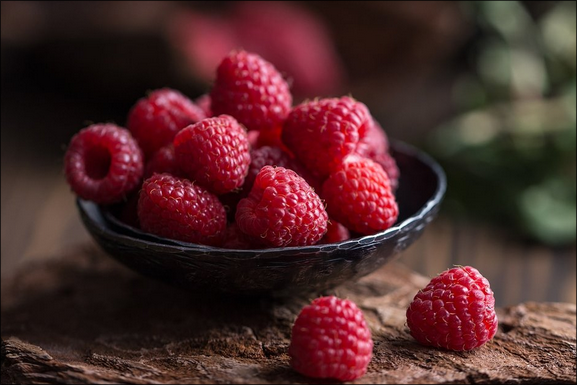
\includegraphics[width=0.5\linewidth]{images/raspberry.png}
        \caption{Because summers are here and we wanted to do something fruity!}
        \label{fig: raspberry}
    \end{figure}
  \end{block}
\end{frame}
%%%%%%%%%%%%%%%%%%%%%%%%%%%%%%%%%%%%%%%%%%%%%%%%%%%%%%%%%%%%%%%%%%%%%%%%%%%%%%%%%%%%%%%



\section{Reaction Scheme}
\subsection{The Plan:}
\begin{frame}{Reaction Scheme}
\begin{figure}
    \centering
    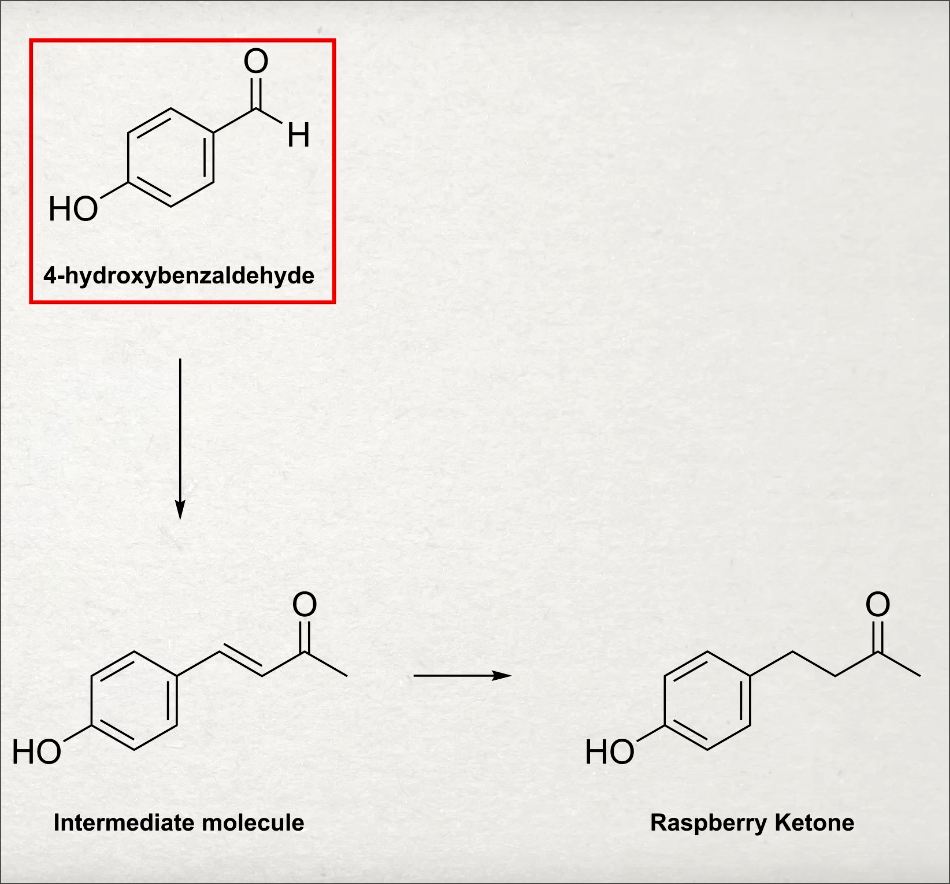
\includegraphics[scale = 0.2]{images/rxn_schme_mini.png}
    \caption{The Base Reaction Scheme that is generally followed\cite{OnePotSynthesisRK}}
    \label{fig:RXN schmeme}
\end{figure}
    
\end{frame}

\begin{frame}{Reaction Scheme}
\begin{figure}
    \centering
    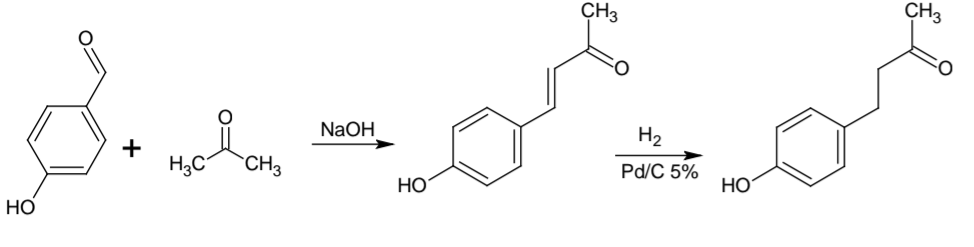
\includegraphics[scale = 0.35]{images/Screenshot_20250415-144215_Files by Google~2.png}
    \caption{The Base Reaction Scheme that is generally followed\cite{OnePotSynthesisRK}}
    \label{fig:RXN schmeme}
\end{figure}
\end{frame}
%%%%%%%%%%%%%%%%%%%%%%%%%%%%%%%%%%%%%%%%%%%%%%%%%%%%%%%%%%%%%%%%%%%%%%%%%%%%%%%%%%%%%%%%%%%%%
\begin{frame}
\frametitle{Synthesis of Rheosmin (Raspberry Ketone)}

\textbf{Procedure:}
\small
\begin{itemize}
    \item Dissolve 10g 4-Hydroxybenzaldehyde in 40ml CaO-dried Propanone with stirring.
    \item \textbf{Slowly} drip in 40ml of 10\% NaOH solution (4g in 40ml water). Let stand overnight to form crystals.
    \item Slurry crystals into 200ml \textbf{ice-cold} 10\% HCl; crystallisation occurs.
    \item Filter and recrystallise from boiling water. (Yield: 5g, MP: 124°C sharp )
    \item \textbf{Hydrogenation Setup:} Flask flushed with \ch{H2}, attached to upturned gas jar filled with \ch{H2}.
    \item Add intermediate product dissolved in 20ml Ethyl Acetate, 5.125g Sodium Acetate, and 0.5g 5\% Pd/C catalyst to the flask.
    \item Stir and allow \ch{H2} absorption (approx. 800ml over 4 hours until absorption ceases). \textit{Note: Large \ch{H2} uptake may indicate leaks.}
    \item Once absorption stops, \textbf{vacuum filter under Nitrogen flow} to recover catalyst.
    \item Wash filtrate with 2x20ml Water to remove Sodium Acetate.
    \item Rotavap Ethyl Acetate to yield oil which crystallises.
    \item Recrystallise from 10ml boiling water. (Final Yield: 3.43g, MP: 82°C sharp )
\end{itemize}
\footnotesize
\textbf{Important Points:}
\begin{itemize}
    \item Use CaO-dried Propanone.
    \item Add NaOH solution slowly.
    \item Use ice-cold HCl for quenching.
    \item Ensure proper hydrogenation setup and monitor gas absorption. Be aware of potential leaks.
    \item Filter catalyst under Nitrogen to prevent side reactions/deactivation.
    \item Purify final product by recrystallisation for sharp melting point.
\end{itemize}

\end{frame}
\subsection{The Physical Setup:}
\begin{frame}{The Physical Setup}

\begin{figure}
\centering
\begin{subfigure}{.45\textwidth}
  \centering
  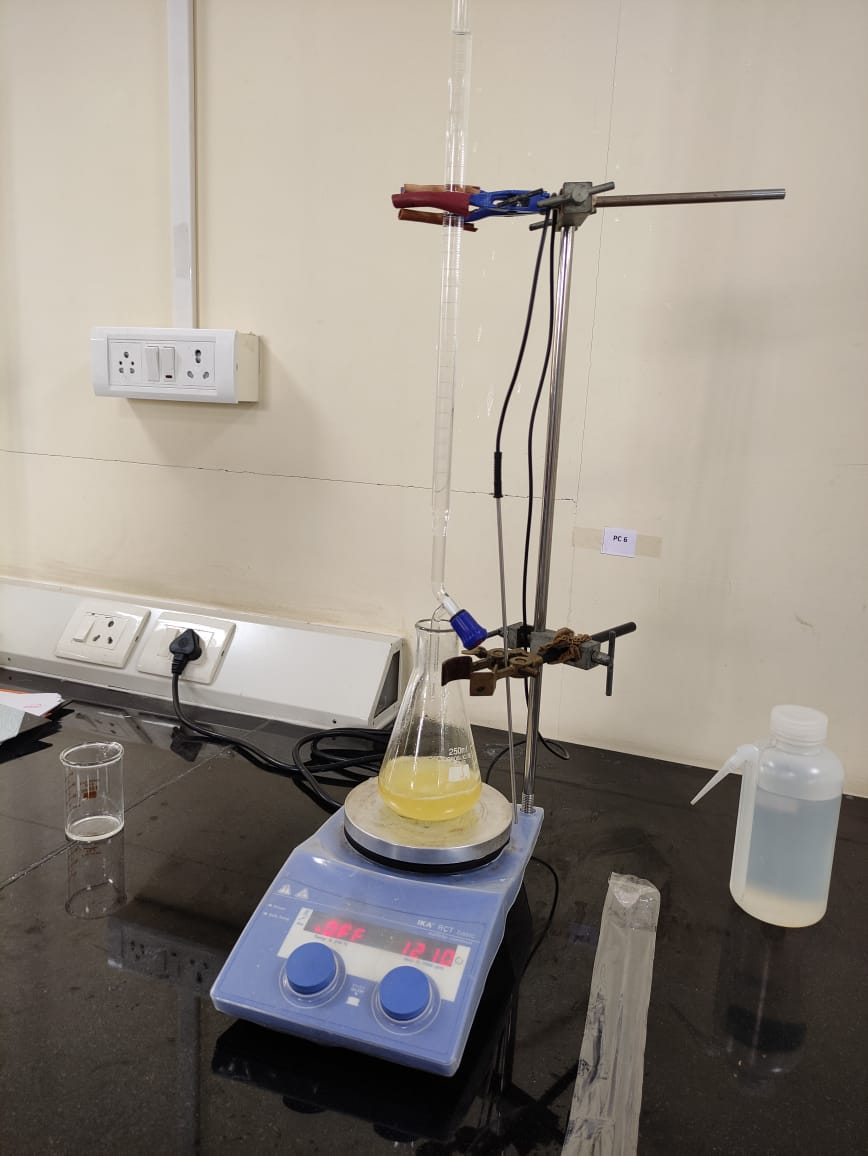
\includegraphics[width=0.62\textwidth]{images/setup_01.png}
  \caption{ The setup consists of the reaction mixture of 10ml 4-methoxybenzaldehyde + 40ml Acetone + 40ml 10\% w/v NaOH solution(in burette)}
  \label{fig:setup01}
\end{subfigure}%
\begin{subfigure}{.45\textwidth}
  \centering
  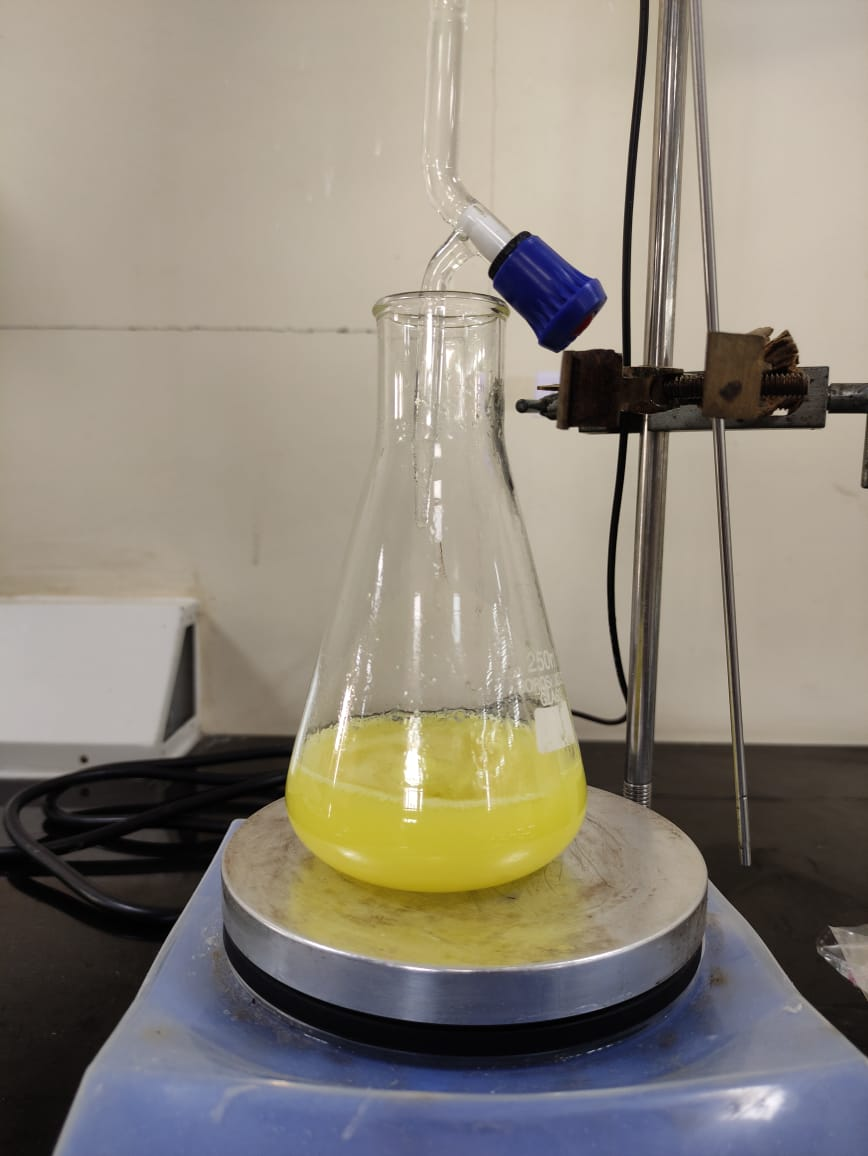
\includegraphics[width=0.62\textwidth]{images/setup_02.png}
  \caption{The Reaction Mixture being stirred vigourously}
  \label{fig:setup02}
\end{subfigure}
\caption{Our Synthesis Setup at the Teaching Lab}
\label{fig:setup}
\end{figure}
\end{frame}

\begin{frame}{The Physical Setup}

\begin{figure}

  \centering
  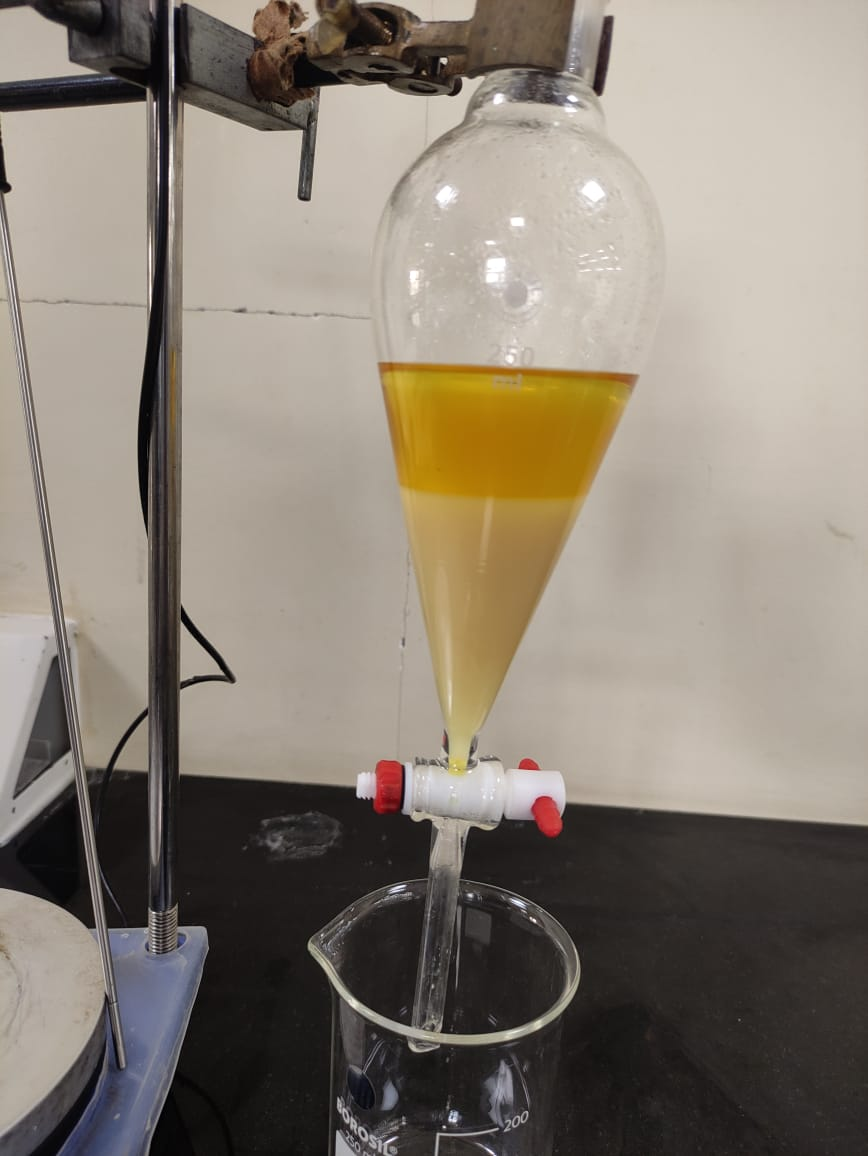
\includegraphics[width=0.3\textwidth]{images/setup_03.png}
  \caption{\centering Separating funnel for separating the aqueous phase \\ from the organic phase (primarily ethyl acetate consisting of the compounds)}

\end{figure}
\end{frame}

%%%%%%%%%%%%%%%%%%%%%%%%%%%%%%%%%%%%%%%%%%%%%%%%%%%%%%%%%%%%%%%%%%%%%%%%%%%%%%%%%%%%%%%%%%%%

\section{Mechanism}
\subsection{Mechanism: Cross Aldol Condensation}
\begin{frame}{Mechanism: Cross Aldol Condensation}
    \begin{figure}
        \centering
        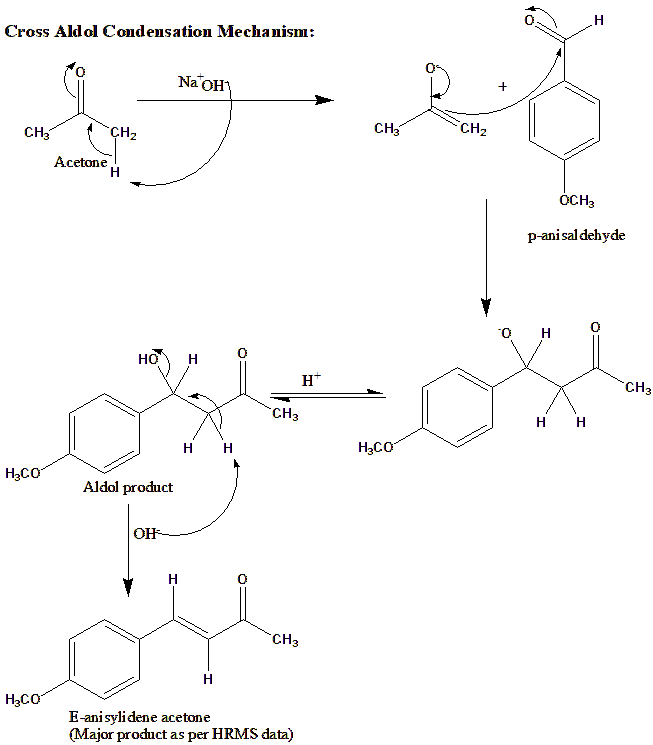
\includegraphics[scale = 0.25]{images/mech.png}
        \caption{Mechanism of the desired product}
        \label{fig:enter-label}
    \end{figure}
\end{frame}

\subsection{Mechanism: So what's the problem?}
\begin{frame}{Mechanism: So what's the problem? }
\begin{figure}
    \centering
    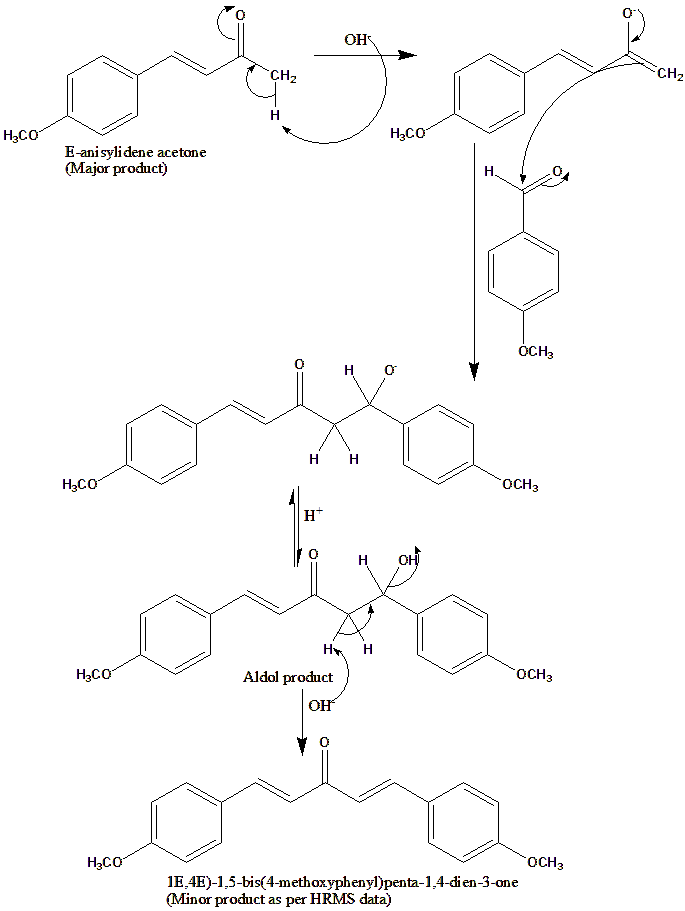
\includegraphics[scale = 0.2]{images/mech_2.png}
    \caption{Mechanism for formation of side product}
    \label{fig:enter-label}
\end{figure}
    
\end{frame}

\begin{frame}{Mechanism}
    \begin{figure}
\centering
\begin{subfigure}{.49\textwidth}
  \centering
  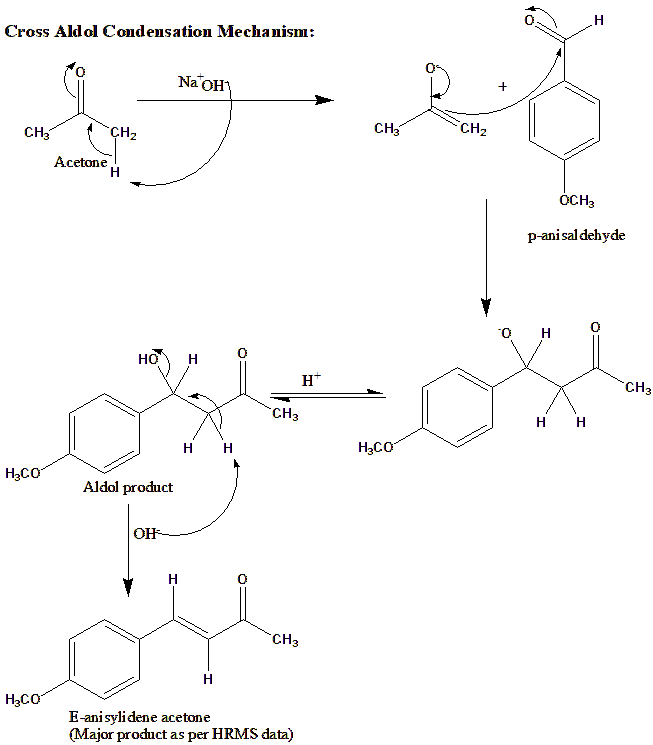
\includegraphics[width=0.65\textwidth]{images/mech.png}
  \caption{ Mechanism of the desired product}
  \label{fig:sub1}
\end{subfigure}%
\begin{subfigure}{.49\textwidth}
  \centering
  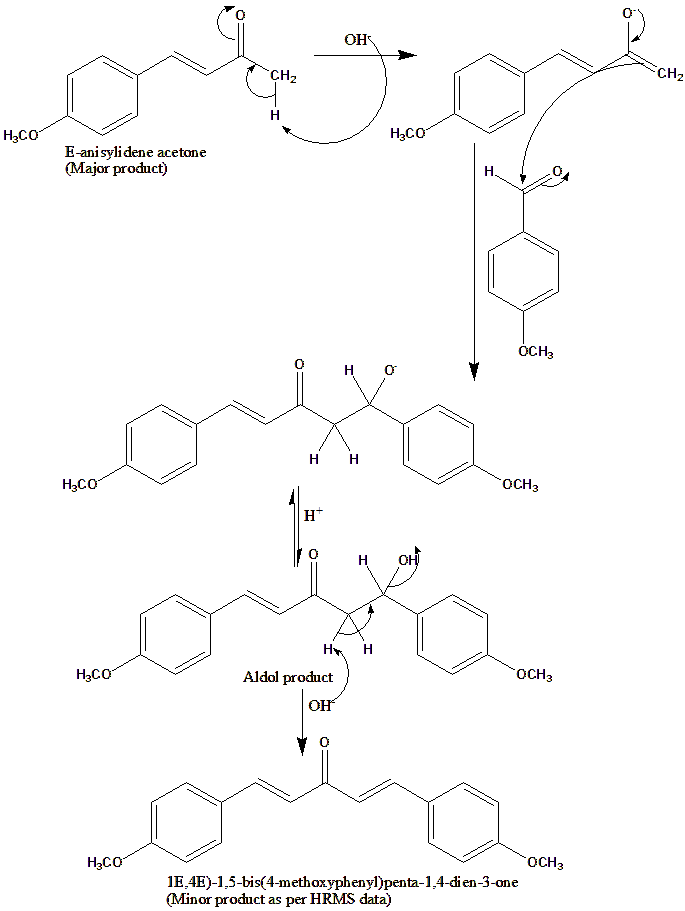
\includegraphics[width=0.5\textwidth]{images/mech_2.png}
  \caption{Mechanism for formation of side product}
  \label{fig:sub2}
\end{subfigure}
\caption{All the Mechanisms shown here were drawn using ChemDrawPro V8.0}
\label{fig:test}
\end{figure}
    
\end{frame}


%%%%%%%%%%%%%%%%%%%%%%%%%%%%%%%%%%%%%%%%%%%%%%%%%%%%%%%%%%%%%%%%%%%%%%%%%%%%%%%%%%%%%%%
\section{Results:}
\subsection{Products Formed}
\subsection{Recrystallization}
\begin{frame}{Results: }
    \begin{figure}
\centering
\begin{subfigure}{.45\textwidth}
  \centering
  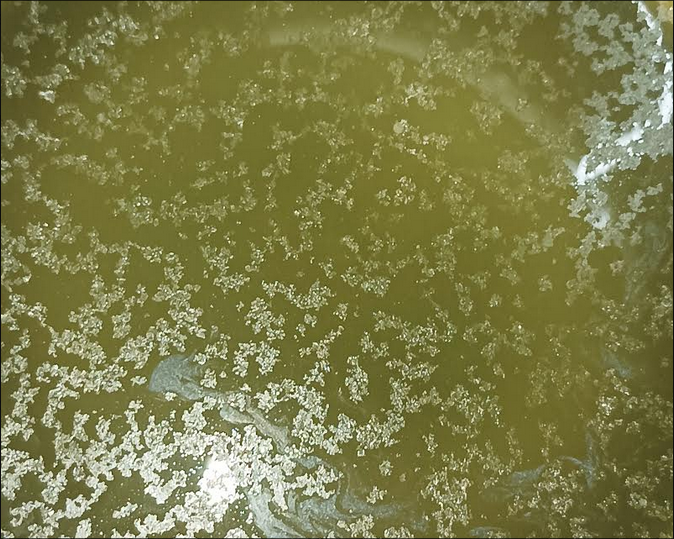
\includegraphics[scale= 0.3]{images/crystallization.png}
  \caption{ Recrystallization in Ethanol}
  \label{fig:sub1}
\end{subfigure}%
\begin{subfigure}{.45\textwidth}
  \centering
  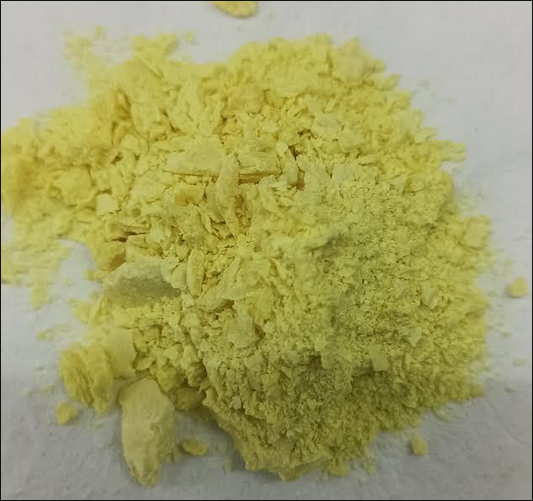
\includegraphics[scale = 0.3]{images/dry_sample.png}
  \caption{The Final Product}
  \label{fig:sub2}
\end{subfigure}
\caption{The Fruit of our Synthesis}
\label{fig:test}
\end{figure}
\end{frame}
%%%%%%%%%%%%%%%%%%%%%%%%%%%%%%%%%%%%%%%%%%%%%%%%%%%%%%%%%%%%%%%%%%%%%%%%%%%%%%%%%%%%%%%
\section{Characterization:}
\subsection{TLC}
\begin{frame}{TLC}
    \begin{figure}
        \centering
        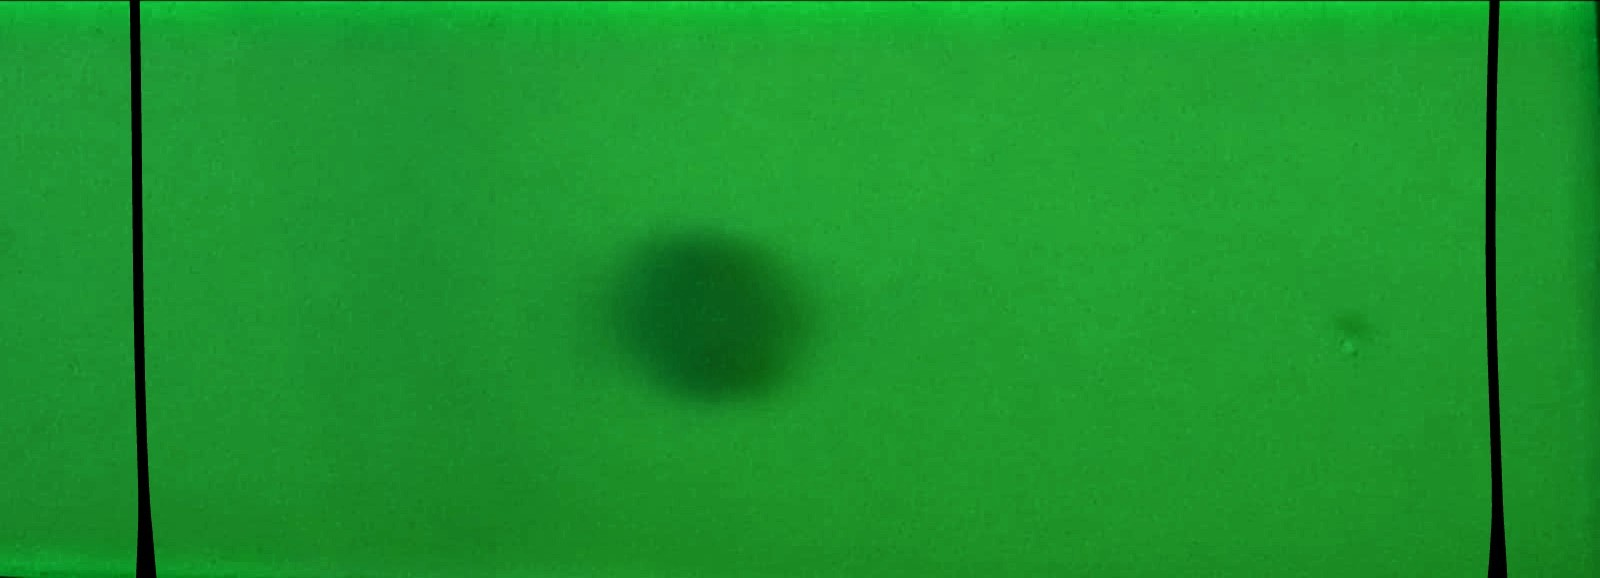
\includegraphics[width=0.8\linewidth]{images/IMG-20250415-WA0042~3.jpg}
        \caption{TLC of the final product mixture in 30\% ethyl acetate in hexane, $R_f$= 0.63}
        \label{fig:enter-label}
    \end{figure}
\end{frame}


\subsection{$^1H$ NMR}
\begin{frame}{Analytical Characterization: $^1$H NMR spectra}
\begin{figure}
    \centering
    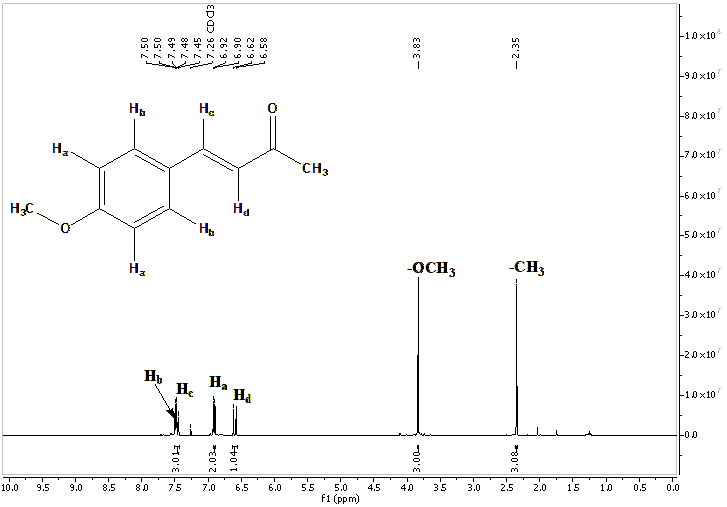
\includegraphics[width=0.6\linewidth]{images/NMR.png}
    \caption{$^1H$ NMR data of the formed product}
    \label{fig:enter-label}
\end{figure}
    
\end{frame}


\subsection{HRMS Data: }
\begin{frame}{Analytical Characterization: HRMS spectra}
\begin{figure}
    \centering
    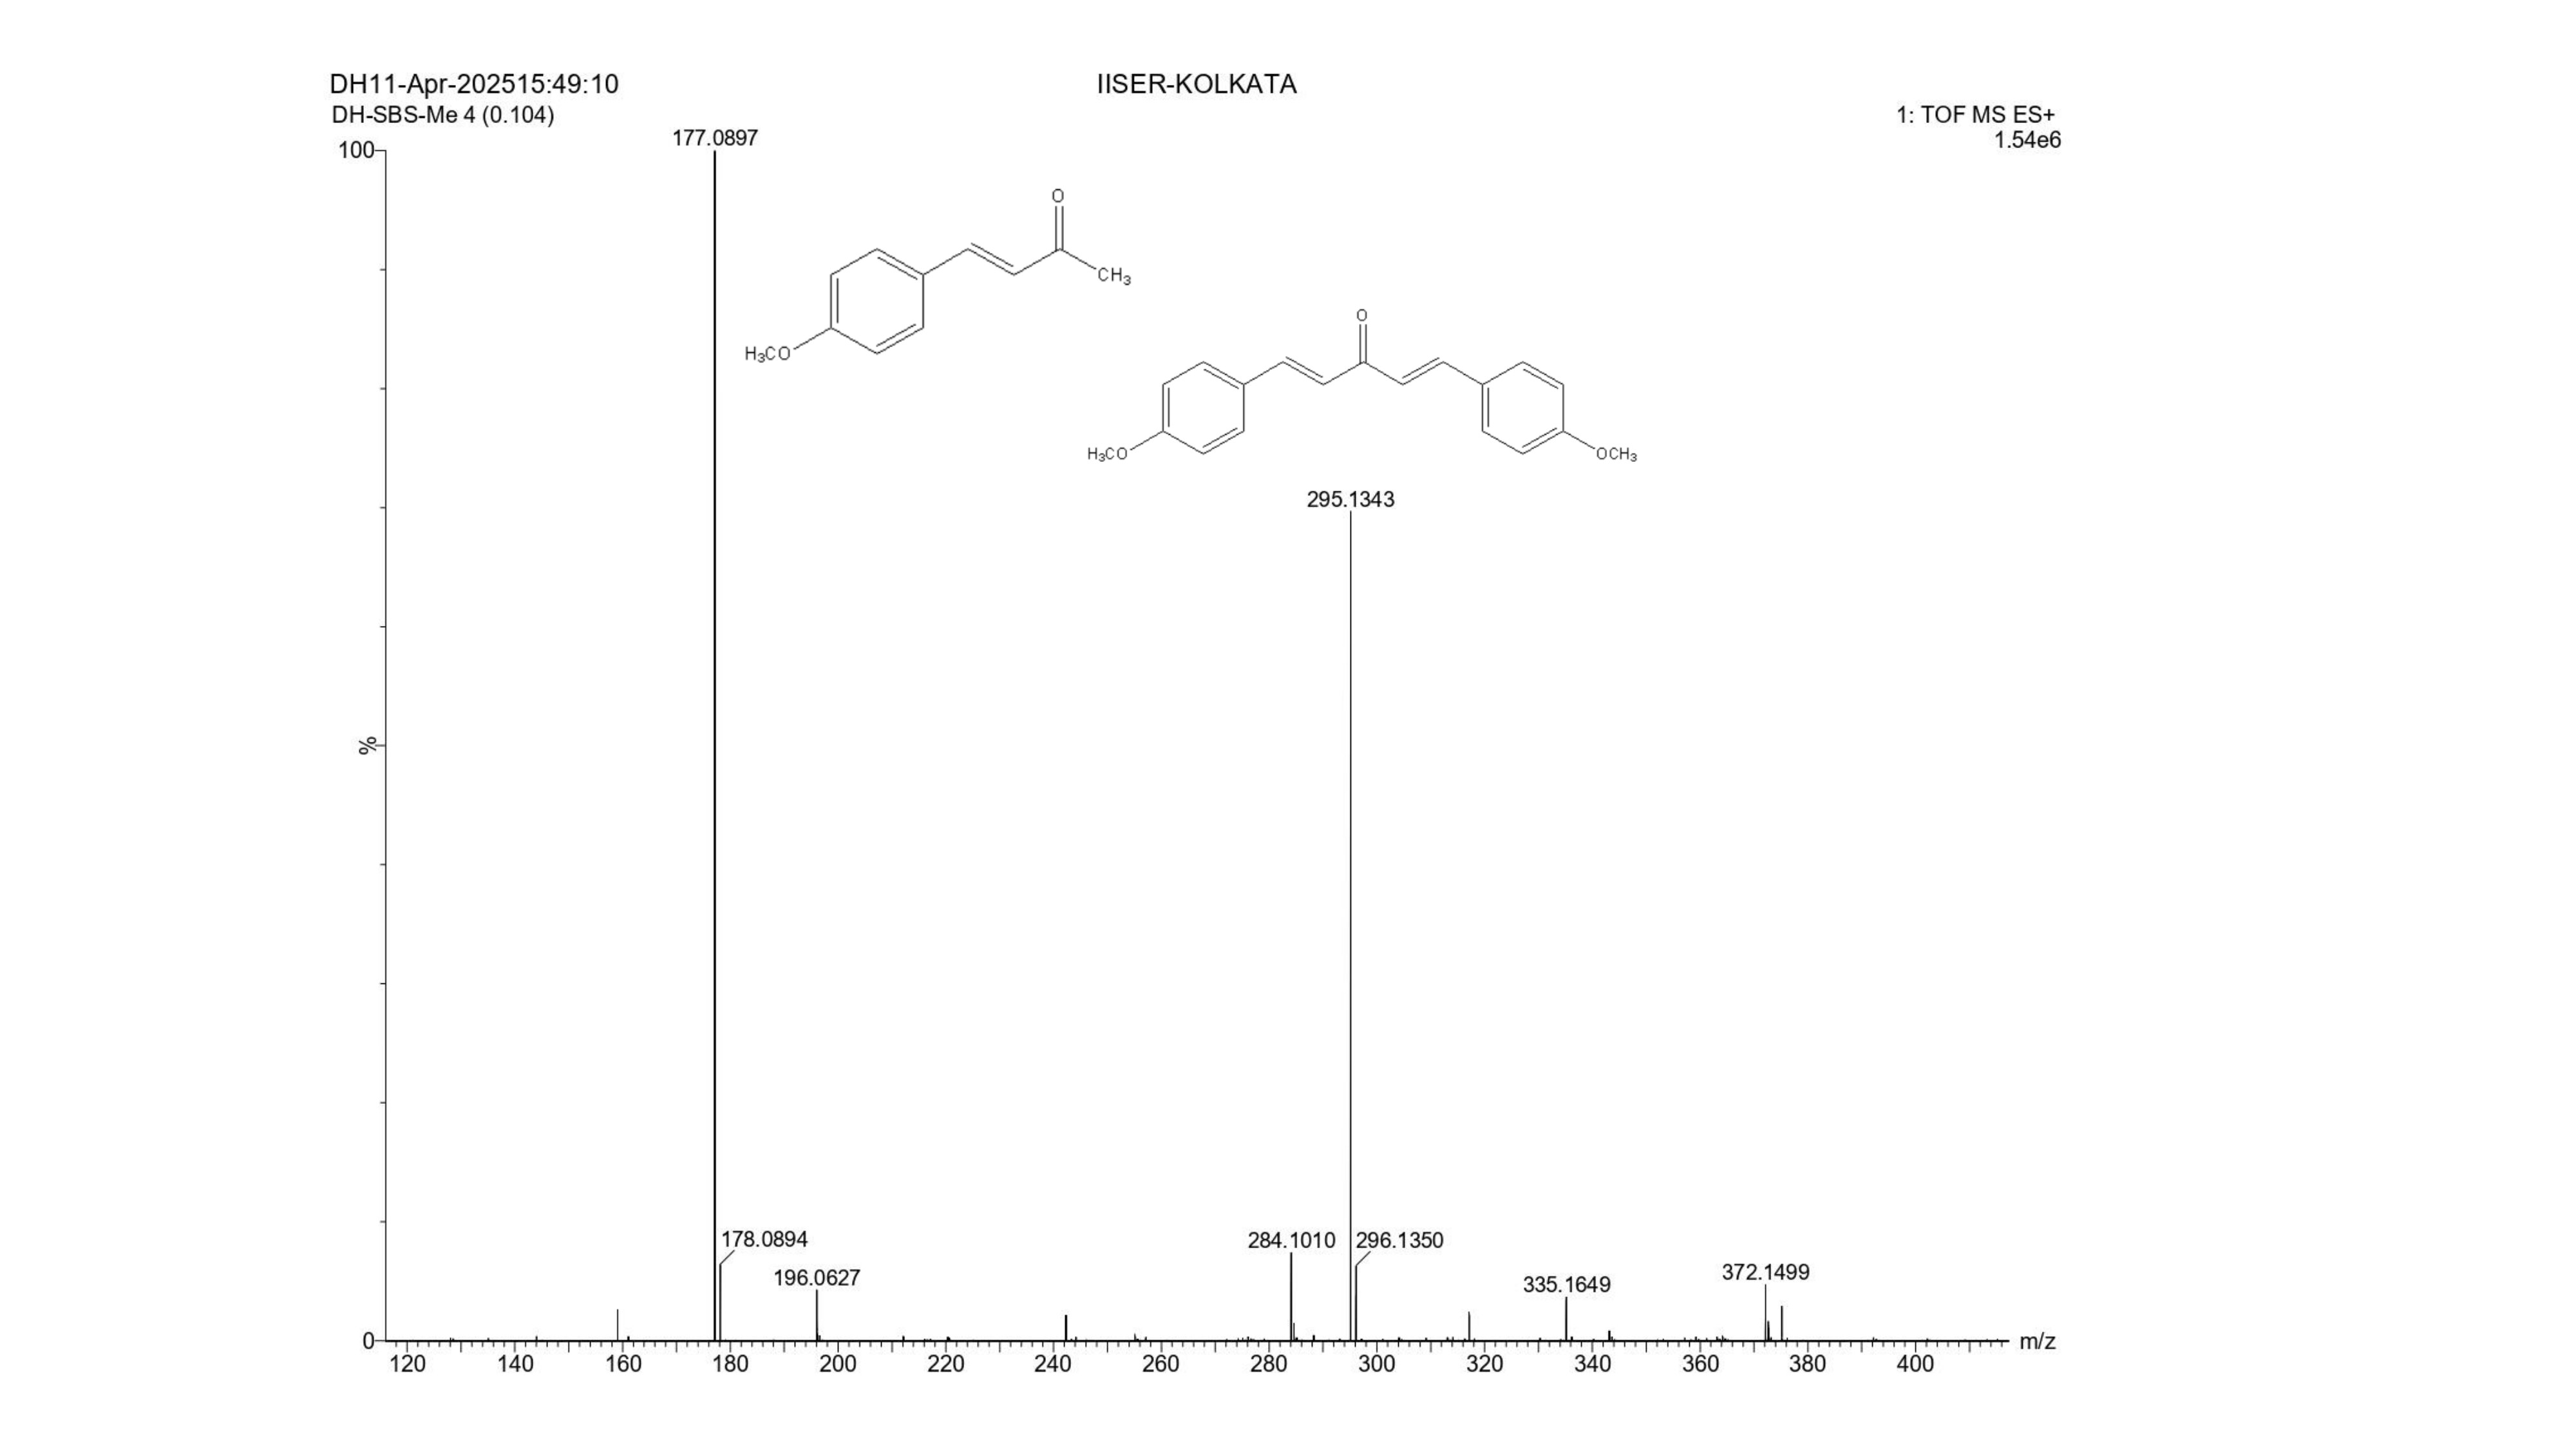
\includegraphics[width=0.8\linewidth]{images/HRMS.jpg}
    \caption{HRMS data of the formed yellow product}
    \label{fig:enter-label}
\end{figure}   
\end{frame}

\subsection{FTIR Data from literature: }
\begin{frame}{Analytical Characterization: FTIR spectra}
\begin{figure}
    \centering
    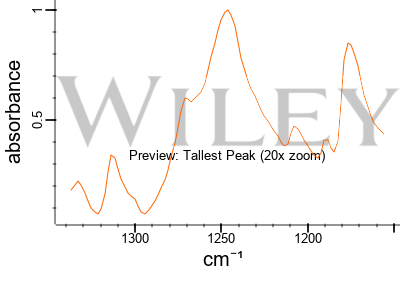
\includegraphics[width=0.5\linewidth]{images/FTIR.png}
    \caption{FTIR data of the major product as per 1989, 1990-2025 Wiley-VCH GmbH}
    \label{fig:FTIR-label}
\end{figure}   
\end{frame}
%%%%%%%%%%%%%%%%%%%%%%%%%%%%%%%%%%%%%%%%%%%%%%%%%%%%%%%%%%%%%%%%%%%%%%%%%%%%%%%%%%%%%%%



%%%%%%%%%%%%%%%%%%%%%%%%%%%%%%%%%%%%%%%%%%%%%%%%%%%%%%%%%%%%%%%%%%%%%%%%%%%%%%%%%%%%%%%
\section{Yield Calculations:}
\begin{frame}{Yield Calculation:}
\textbf{Step 1: Calculate the mass of anisaldehyde used}
\begin{align}
\text{Mass of anisaldehyde} &= \text{Volume} \times \text{Density} \\
&= 10 \text{ mL} \times 1.12 \text{ g/mL} \\
&= 11.2 \text{ g}
\end{align}

\textbf{Step 2: Calculate moles of anisaldehyde used}
\begin{align}
\text{Molar mass of anisaldehyde} &= 136.15 \text{ g/mol} \\
\text{Moles of anisaldehyde} &= \frac{11.2 \text{ g}}{136.15 \text{ g/mol}} \\
&= 0.0823 \text{ mol}
\end{align}

\textbf{Step 3: Define variables}
\begin{align}
x &= \text{moles of major product} \\
0.7x &= \text{moles of minor product (from 10:7 ratio)}
\end{align}
\end{frame}
\begin{frame}{Yield Calculation:}
    

\textbf{Step 4: Set up equations based on anisaldehyde consumption}
\begin{align}
\text{Anisaldehyde for major product} &= x \text{ mol} \\
\text{Anisaldehyde for minor product} &= 2 \times 0.7x = 1.4x \text{ mol} \\
\text{Total anisaldehyde used} &= x + 1.4x = 2.4x \text{ mol}
\end{align}

\textbf{Step 5: Solve for x using the total anisaldehyde amount}
\begin{align}
2.4x &= 0.0823 \\
x &= \frac{0.0823}{2.4} \\
x &= 0.03429 \text{ mol}
\end{align}

\textbf{Step 6: Calculate moles of each product}
\begin{align}
\text{Moles of major product} &= x = 0.03429 \text{ mol} \\
\text{Moles of minor product} &= 0.7x = 0.7 \times 0.03429 = 0.02400 \text{ mol}
\end{align}
\end{frame}
\begin{frame}{Yield Calculation:}
\textbf{Step 7: Calculate actual yield of each product}
\begin{align}
\text{Mass of major product} &= 0.03429 \text{ mol} \times 177.0897 \text{ g/mol} \\
&= 6.073 \text{ g} \\
\text{Mass of minor product} &= 0.02400 \text{ mol} \times 295.1343 \text{ g/mol} \\
&= 7.083 \text{ g} \\
\text{Total mass of products} &= 6.073 \text{ g} + 7.083 \text{ g} = 13.156 \text{ g}
\end{align}

\textbf{Step 8: Adjust calculation based on the actual total yield}
\begin{align}
\text{Actual total yield} &= 11.564 \text{ g} \\
\text{Correction factor} &= \frac{11.564}{13.156} = 0.8790 \\
\text{Actual major product yield} &= 6.073 \times 0.8790 = 5.338 \text{ g} \\
\text{Actual minor product yield} &= 7.083 \times 0.8790 = 6.226 \text{ g}
\end{align}
\end{frame}

\begin{frame}{Yield Calculation:}
\textbf{Step 9: Calculate theoretical yields}
\begin{align}
\text{For major product:} \\
\text{Maximum moles from anisaldehyde} &= 0.0823 \text{ mol} \\
\text{Theoretical yield} &= 0.0823 \text{ mol} \times 177.0897 \text{ g/mol} \\
&= 14.574 \text{ g} \\
\text{For minor product:} \\
\text{Maximum moles from anisaldehyde} &= \frac{0.0823 \text{ mol}}{2} = 0.04115 \text{ mol} \\
\text{Theoretical yield} &= 0.04115 \text{ mol} \times 295.1343 \text{ g/mol} \\
&= 12.145 \text{ g}
\end{align}
\end{frame}
\begin{frame}{Yield Calculation:}
\textbf{Step 10: Calculate percent yields}
\begin{align}
\text{\% Yield of major product} &= \frac{\text{Actual yield}}{\text{Theoretical yield}} \times 100\% \\
&= \frac{5.338 \text{ g}}{14.574 \text{ g}} \times 100\% \\
&= 36.63\% \\
\text{\% Yield of minor product} &= \frac{\text{Actual yield}}{\text{Theoretical yield}} \times 100\% \\
&= \frac{6.226 \text{ g}}{12.145 \text{ g}} \times 100\% \\
&= 51.26\%
\end{align}

\textbf{Final Answer:}
\begin{align}
\text{\% Yield of major product} &= 36.63\% \\
\text{\% Yield of minor product} &= 51.26\%
\end{align}
    
\end{frame}
%%%%%%%%%%%%%%%%%%%%%%%%%%%%%%%%%%%%%%%%%%%%%%%%%%%%%%%%%%%%%%%%%%%%%%%%%%%%%%%%%%%%%%%%%%%%

\section{Computational Analysis: }

\begin{frame}
\frametitle{Computational Parameters for Anisylidene Acetone}
\begin{center}
\fbox{
\begin{minipage}{0.9\textwidth}

# opt freq b3lyp/6-311g scrf=(iefpcm,solvent=acetone) guess=save 
pop=(mk,nto,savento,savemulliken) density=current geom=connectivity

\end{minipage}
}
\end{center}

\vspace{0.1cm}
\begin{description}[labelwidth=2.5cm, leftmargin=!]
\item[opt] Geometry optimization to find the minimum energy structure
\item[freq] Calculate vibrational frequencies for thermodynamic properties and confirm stationary point
\item[b3lyp] Becke's three-parameter hybrid functional with Lee-Yang-Parr correlation
\item[6-311g] Split-valence triple-zeta basis set with polarization functions
\item[scrf] Self-Consistent Reaction Field for solvation effects
\item[iefpcm] Integral Equation Formalism Polarizable Continuum Model
\item[solvent] Acetone as the solvent environment
\item[guess=save] Save the converged wavefunction for future calculations
\item[pop=mk] Merz-Kollman scheme for calculating atomic charges
\item[nto] Natural Transition Orbitals analysis
\item[savento] Save the Natural Transition Orbitals
\item[savemulliken] Save the Mulliken population analysis
\item[density=current] Use the current density matrix for population analysis
\item[geom=connectivity] Include molecular connectivity in the input file
\end{description}
\end{frame}


\begin{frame}{HOMO Visualization}
         \begin{figure}
\centering
\begin{subfigure}{.49\textwidth}
  \centering
  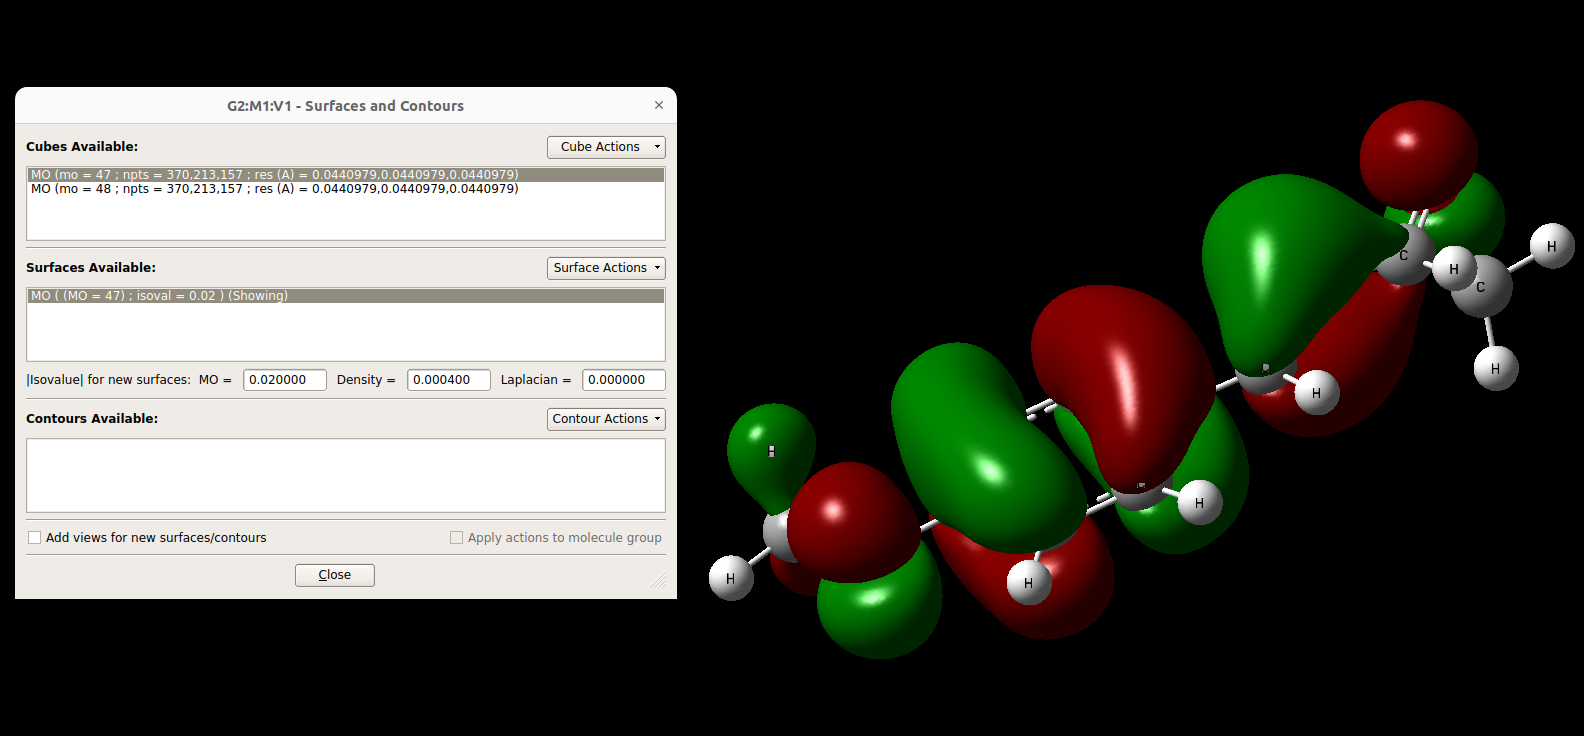
\includegraphics[width=0.9\textwidth]{images/HOMO_01.png}
  % \caption{A Side View of Solvation Cavity}
  \label{fig:sub1}
\end{subfigure}%
\begin{subfigure}{.49\textwidth}
  \centering
  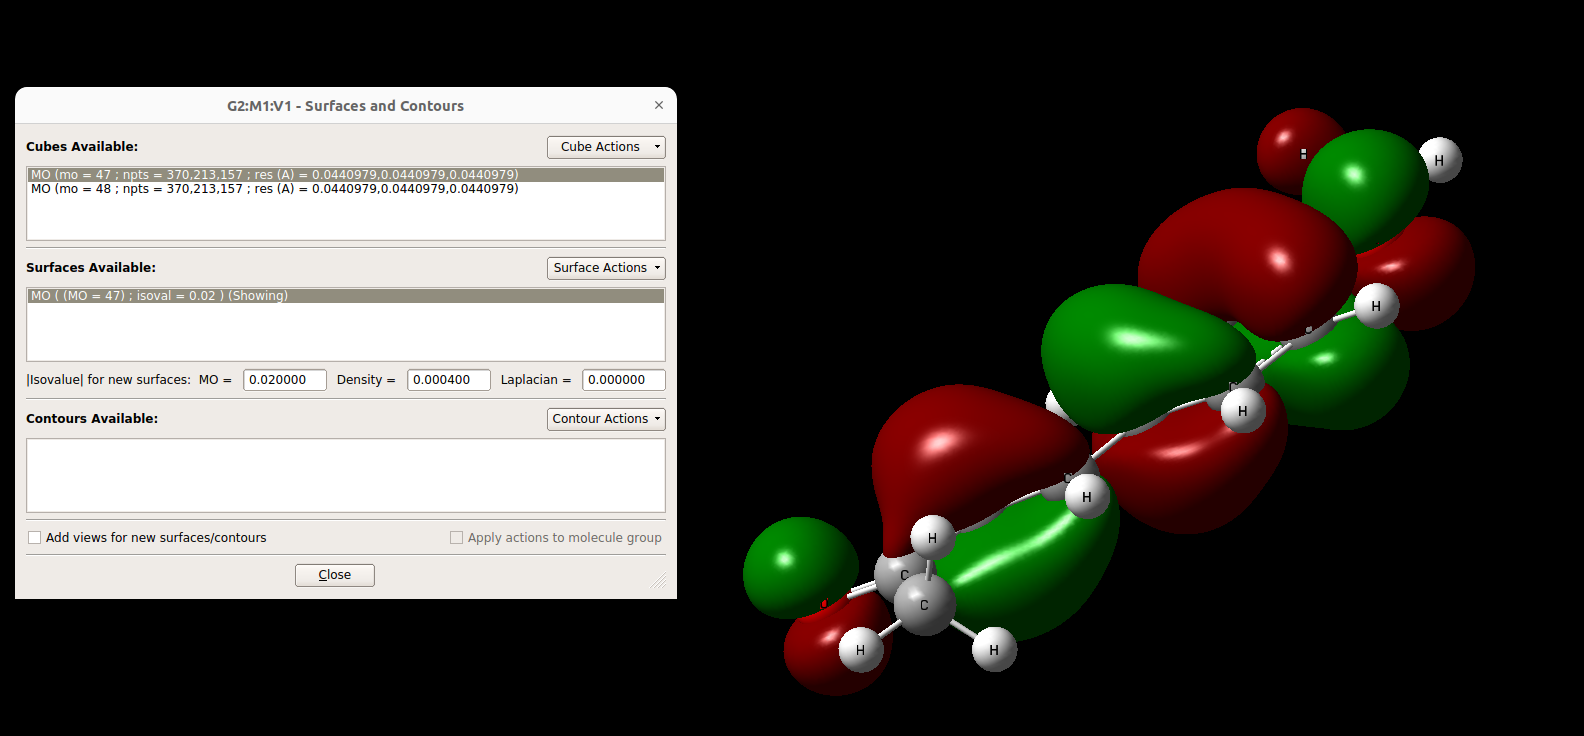
\includegraphics[width=0.9\textwidth]{images/HOMO_02.png}
  % \caption{A $\frac{3}{4}^{th}$ view of the Solvation Cavity}
  \label{fig:sub2}
\end{subfigure}
\caption{Visualizing the HOMO}
\label{fig:test}
\end{figure}
\end{frame}

\begin{frame}{LUMO Visualization}
         \begin{figure}
\centering
\begin{subfigure}{.49\textwidth}
  \centering
  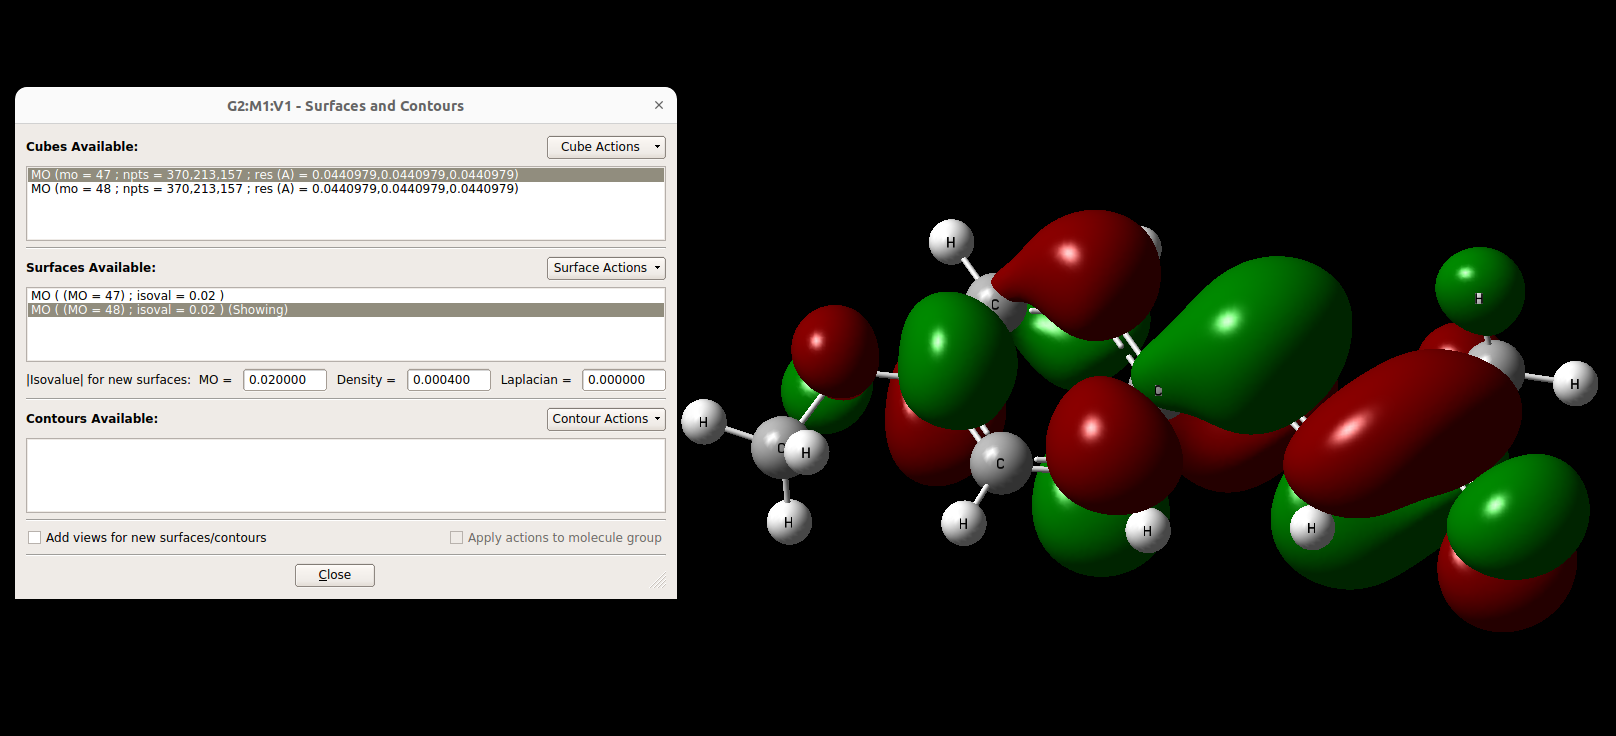
\includegraphics[width=0.9\textwidth]{images/LUMO_01.png}
  % \caption{A Side View of Solvation Cavity}
  \label{fig:sub1}
\end{subfigure}%
\begin{subfigure}{.49\textwidth}
  \centering
  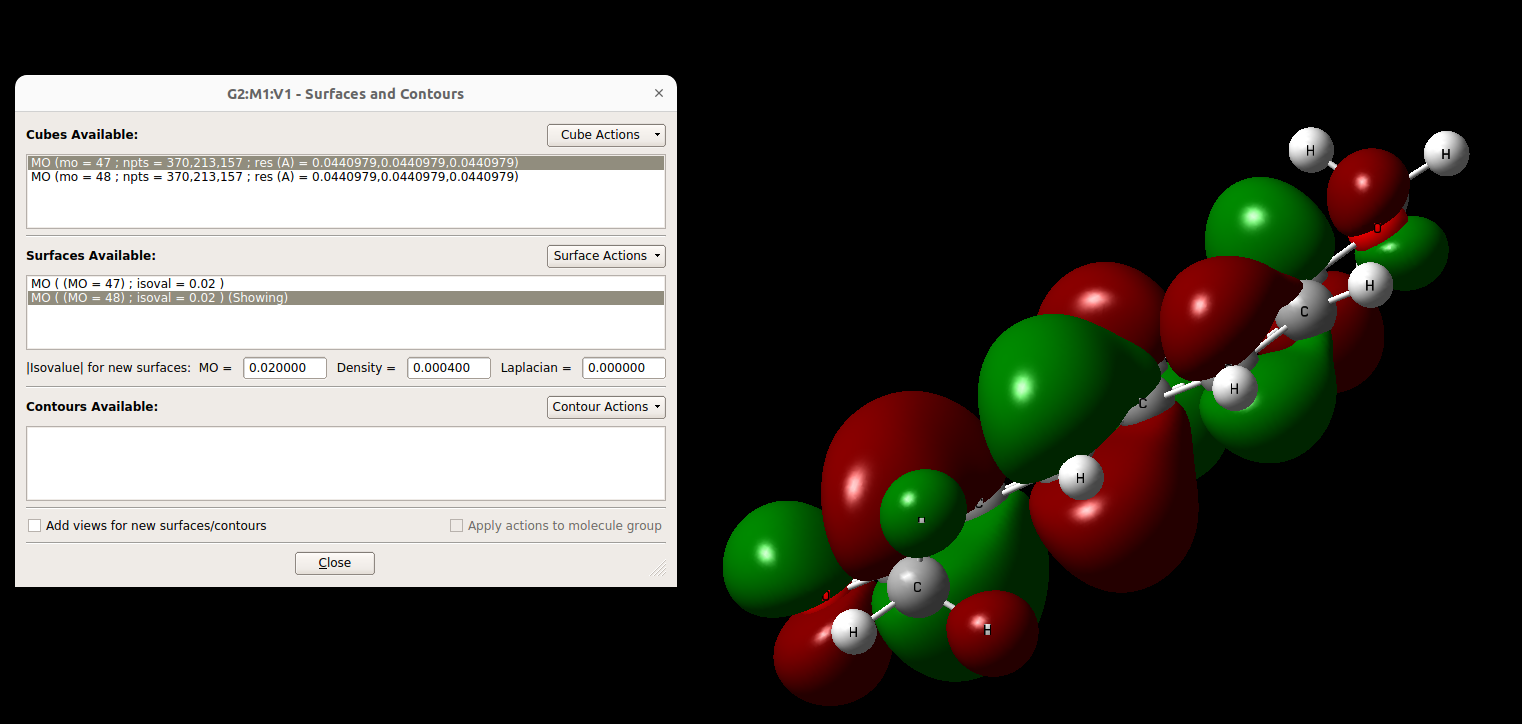
\includegraphics[width=0.9\textwidth]{images/LUMO_02.png}
  % \caption{A $\frac{3}{4}^{th}$ view of the Solvation Cavity}
  \label{fig:sub2}
\end{subfigure}
\caption{Visualizing the LUMO}
\label{fig:test}
\end{figure}
\end{frame}


\begin{frame}{HOMO-LUMO Gap}
    \begin{figure}
        \centering
        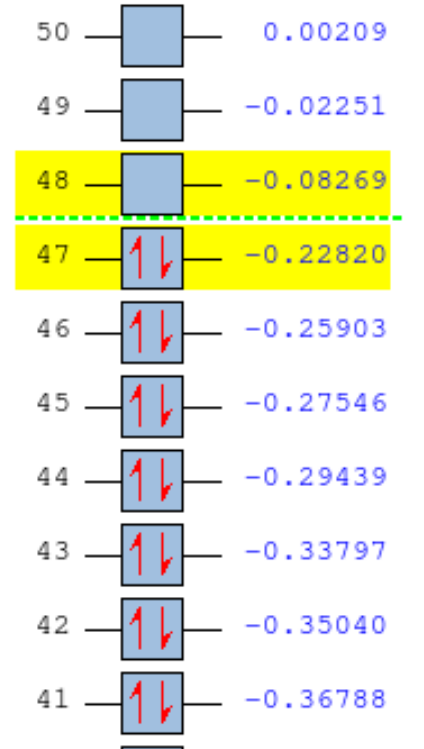
\includegraphics[width=0.2\linewidth]{images/homo_lumo.png}
        \caption{The HOMO-LUMO Energy Gap in Hartree}
        \label{fig: HOMO-LUMO Gap}
    \end{figure}
\end{frame}



\begin{frame}
\frametitle{Rotational Properties of Anisylidene Acetone}
\begin{columns}
\begin{column}{0.6\textwidth}
\begin{center}
\begin{tabular}{|l|c|c|c|}
\hline
\textbf{Principal Axis} & \textbf{1} & \textbf{2} & \textbf{3} \\
\hline
Moment of Inertia (a.u.) & 633.31 & 6425.00 & 7035.65 \\
\hline
Rotational Temp. (K) & 0.137 & 0.013 & 0.012 \\
\hline
Rotational Const. (GHz) & 2.850 & 0.281 & 0.257 \\
\hline
\end{tabular}
\end{center}
\end{column}
\begin{column}{0.4\textwidth}
\begin{itemize}
\item Classified as an asymmetric top
\item Rotational symmetry number: 1
\item Significant difference between axis 1 vs. axes 2 \& 3
\item Near-planar orientation (X-Y plane)
\item Principal axes nearly aligned with Cartesian axes
\end{itemize}
\end{column}
\end{columns}
\end{frame}

\begin{frame}
\frametitle{Vibrational Properties - Zero-Point Energy}
\begin{columns}
\begin{column}{0.55\textwidth}
\begin{center}
\begin{tabular}{|l|c|}
\hline
\textbf{Zero-Point Energy} & \textbf{Value} \\
\hline
Joules/Mol & 535,326.2 \\
\hline
Kcal/Mol & 127.95 \\
\hline
Hartree/Particle & 0.203895 \\
\hline
\end{tabular}
\end{center}
\end{column}
\begin{column}{0.45\textwidth}
\begin{itemize}
\item Significant ZPE reflects:
  \begin{itemize}
  \item Large molecular size
  \item Multiple vibrational modes (69 total)
  \item Presence of high-frequency C-H stretches
  \end{itemize}
\item 19 degrees of freedom considered as vibrations
\end{itemize}
\end{column}
\end{columns}
\end{frame}

\begin{frame}
\frametitle{Vibrational Temperature Distribution}
\begin{columns}
\begin{column}{0.55\textwidth}
\begin{center}
\begin{tabular}{|l|c|}
\hline
\textbf{Vibrational Temp. Range (K)} & \textbf{Interpretation} \\
\hline
54-200 & Low-frequency modes \\
\hline
200-1000 & Framework vibrations \\
\hline
1000-2000 & Stretching vibrations \\
\hline
2000-3000 & Double-bond stretching \\
\hline
4300-4650 & C-H stretching modes \\
\hline
\end{tabular}
\end{center}
\end{column}
\begin{column}{0.45\textwidth}
\begin{itemize}
\item Low-frequency modes:
  \begin{itemize}
  \item Torsional motions
  \item Ring deformations
  \end{itemize}
\item Mid-range frequencies:
  \begin{itemize}
  \item C-C stretching
  \item C=C ring modes
  \end{itemize}
\item High frequencies:
  \begin{itemize}
  \item C-H stretching
  \item Characteristic of aromatic systems
  \end{itemize}
\end{itemize}
\end{column}
\end{columns}
\end{frame}

\begin{frame}
\frametitle{Thermodynamic Properties}
\begin{center}
\begin{tabular}{|l|c|}
\hline
\textbf{Property} & \textbf{Value (Hartree)} \\
\hline
Zero-point correction & 0.203895 \\
\hline
Thermal correction to Energy & 0.216654 \\
\hline
Thermal correction to Enthalpy & 0.217598 \\
\hline
Thermal correction to Gibbs Free Energy & 0.163613 \\
\hline
Sum of electronic and zero-point Energies & -576.612812 \\
\hline
Sum of electronic and thermal Energies & -576.600052 \\
\hline
Sum of electronic and thermal Enthalpies & -576.599108 \\
\hline
Sum of electronic and thermal Free Energies & -576.653093 \\
\hline
\end{tabular}
\end{center}
\end{frame}

\begin{frame}
\frametitle{Thermodynamic Analysis}
\begin{columns}
\begin{column}{0.48\textwidth}
\textbf{Key Insights:}
\begin{itemize}
\item Significant entropic contribution 
  \begin{itemize}
  \item T$\Delta$S = 0.053985 Hartree
  \item ≈ 33.9 kcal/mol at 298K
  \end{itemize}
\item Thermal energy contribution
  \begin{itemize}
  \item E$_{thermal}$ - E$_{ZPE}$ = 0.012759 Hartree
  \item ≈ 8.0 kcal/mol
  \end{itemize}  
\end{itemize}
\end{column}
\begin{column}{0.52\textwidth}
\textbf{Implications:}
\begin{itemize}
\item Conformational flexibility
  \begin{itemize}
  \item Possible rotations around C-C bonds
  \item Multiple accessible conformers
  \end{itemize}
\item Reaction thermodynamics
  \begin{itemize}
  \item Free energy guidance for reactions
  \item Significant entropic effects
  \item Temperature-dependent stability
  \end{itemize}
\end{itemize}
\end{column}
\end{columns}
\end{frame}

\begin{frame}
\frametitle{Structure-Dynamics Relationships}
\begin{itemize}
\item Molecular shape characterization:
  \begin{itemize}
  \item Elongated structure (I$_1$ ≪ I$_2$ ≈ I$_3$)
  \item Nearly planar configuration
  \item Rotational constants suggest restricted rotation
  \end{itemize}
\item Vibrational signature highlights:
  \begin{itemize}
  \item Conjugated system (characteristic frequencies)
  \item Functional group identification (carbonyl, methoxy)
  \item Framework rigidity (high-frequency skeletal modes)
  \end{itemize}
\item Thermodynamic behavior:
  \begin{itemize}
  \item Entropic stabilization at higher temperatures
  \item Enthalpic stability from conjugation
  \item Thermal mobility of side groups
  \end{itemize}
\end{itemize}
\end{frame}
\begin{frame}
\frametitle{Electric Dipole Moment of Anisylidene Acetone}
\begin{columns}
\begin{column}{0.6\textwidth}
\begin{center}
\begin{tabular}{|l|c|c|}
\hline
\textbf{Component} & \textbf{Magnitude (Debye)} & \textbf{Direction} \\
\hline
Total & 6.13 & -- \\
\hline
X & -0.89 & Weak contribution \\
\hline
Y & -5.85 & Major contributor \\
\hline
Z & 1.59 & Moderate contribution \\
\hline
\end{tabular}
\end{center}
\end{column}
\begin{column}{0.4\textwidth}
\begin{itemize}
\item Significant total dipole moment (6.13 D)
\item Strong Y-axis polarization
\item Suggests highly asymmetric charge distribution
\item Characteristic of conjugated systems with electron-withdrawing groups
\end{itemize}
\end{column}
\end{columns}
\end{frame}

\begin{frame}
\frametitle{Polarizability Analysis}
\begin{columns}
\begin{column}{0.5\textwidth}
\begin{center}
\begin{tabular}{|l|c|}
\hline
\textbf{Property} & \textbf{Value ($\times 10^{-24}$ esu)} \\
\hline
Isotropic $\alpha$ & 28.51 \\
\hline
Anisotropic $\alpha$ & 34.25 \\
\hline
\end{tabular}

\vspace{0.5cm}

\begin{tabular}{|l|c|}
\hline
\textbf{Component} & \textbf{Value ($\times 10^{-24}$ esu)} \\
\hline
$\alpha_{xx}$ & 26.21 \\
\hline
$\alpha_{yy}$ & 45.35 \\
\hline
$\alpha_{zz}$ & 13.98 \\
\hline
\end{tabular}
\end{center}
\end{column}
\begin{column}{0.5\textwidth}
\begin{itemize}
\item High anisotropy ratio (1.20)
\item Dominant Y-axis polarizability
\item X-axis - moderate response
\item Z-axis - least polarizable
\item Aligns with molecular structure:
  \begin{itemize}
  \item Y-axis spans conjugated system
  \item Z-axis perpendicular to aromatic plane
  \end{itemize}
\end{itemize}
\end{column}
\end{columns}
\end{frame}

\begin{frame}
\frametitle{Dipole Orientation Analysis}
\begin{columns}
\begin{column}{0.55\textwidth}
\centering
\begin{tabular}{|l|c|c|}
\hline
\textbf{Component} & \textbf{Input} & \textbf{Dipole} \\
\textbf{} & \textbf{Orientation (D)} & \textbf{Orientation (D)} \\
\hline
Total & 6.13 & 6.13 \\
\hline
X & -0.89 & 0.00 \\
\hline
Y & -5.85 & 0.00 \\
\hline
Z & 1.59 & 6.13 \\
\hline
\end{tabular}
\end{column}
\begin{column}{0.45\textwidth}
\begin{itemize}
\item In dipole orientation:
  \begin{itemize}
  \item Z-axis aligns with molecular dipole
  \item X and Y components vanish
  \end{itemize}
\item Dipole direction indicates electron density distribution
\item Points from electron-rich methoxy group toward carbonyl moiety
\end{itemize}
\end{column}
\end{columns}
\end{frame}

\begin{frame}
\frametitle{Structure-Property Relationships}
\begin{columns}
\begin{column}{0.48\textwidth}
\centering
\textbf{Key Insights:}
\begin{itemize}
\item High polarizability ($\alpha_{iso} = 28.51 \times 10^{-24}$ esu)
\item Significant dipole moment (6.13 D)
\item Strong anisotropy in both properties
\end{itemize}

\vspace{0.3cm}
\textbf{Contributing Factors:}
\begin{itemize}
\item Conjugated π-system
\item Electron-donating methoxy group
\item Electron-withdrawing carbonyl group
\end{itemize}
\end{column}
\begin{column}{0.52\textwidth}
\textbf{Implications for Molecular Properties:}
\begin{itemize}
\item Enhanced solubility in polar solvents
\item Strong intermolecular interactions
\item Potential for hydrogen bonding
\item Significant reactivity at carbonyl center
\item Possible π-stacking interactions
\item UV-vis absorption characteristics
\end{itemize}
\end{column}
\end{columns}
\end{frame}

\begin{frame}{PCM Solvation Cavity}
     \begin{figure}
\centering
\begin{subfigure}{.49\textwidth}
  \centering
  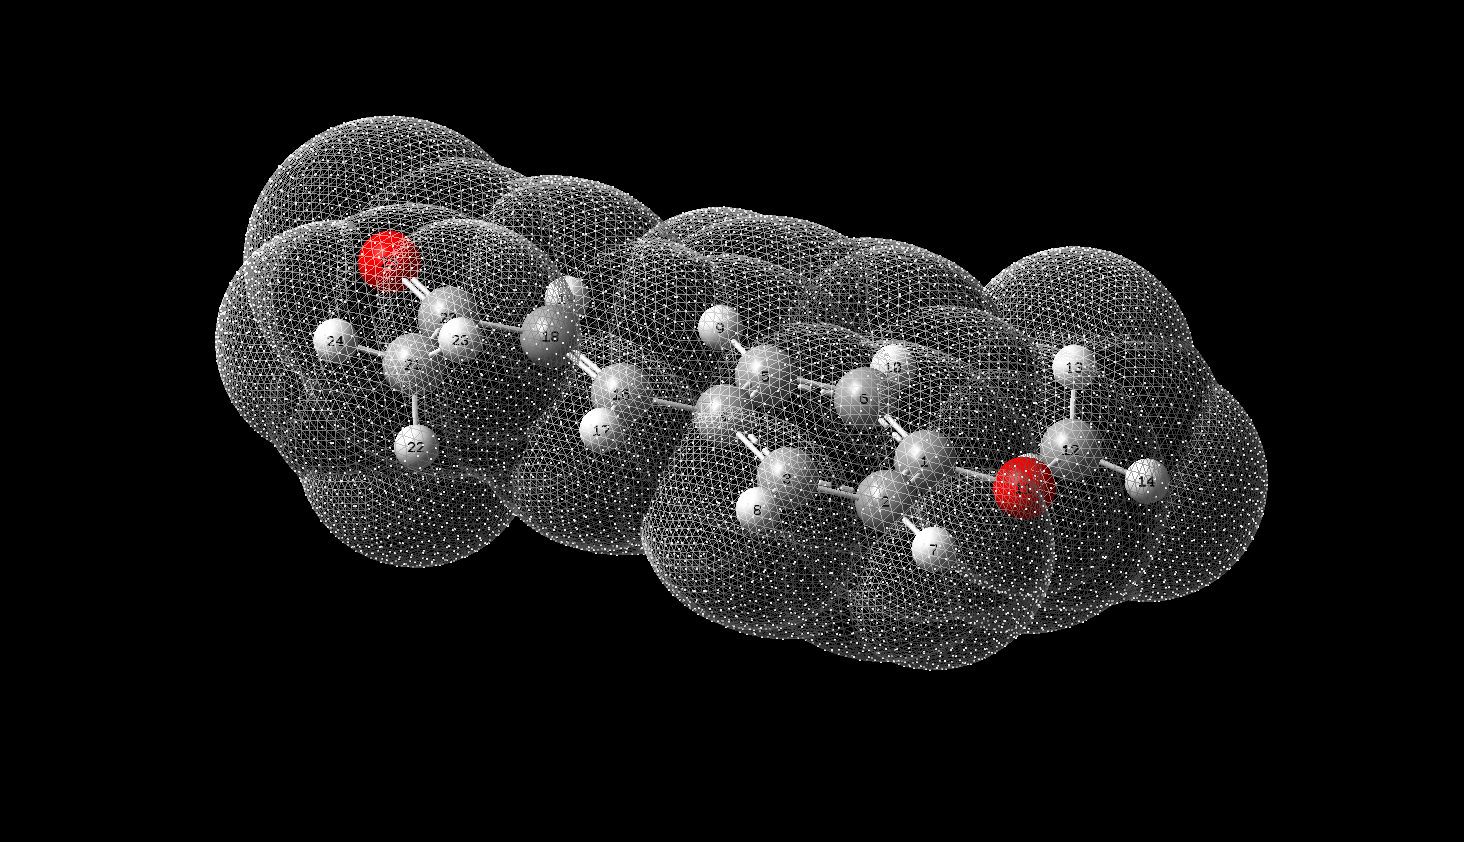
\includegraphics[width=0.85\textwidth]{images/solvation_cavity_01.png}
  \caption{A Side View of Solvation Cavity}
  \label{fig:sub1}
\end{subfigure}%
\begin{subfigure}{.49\textwidth}
  \centering
  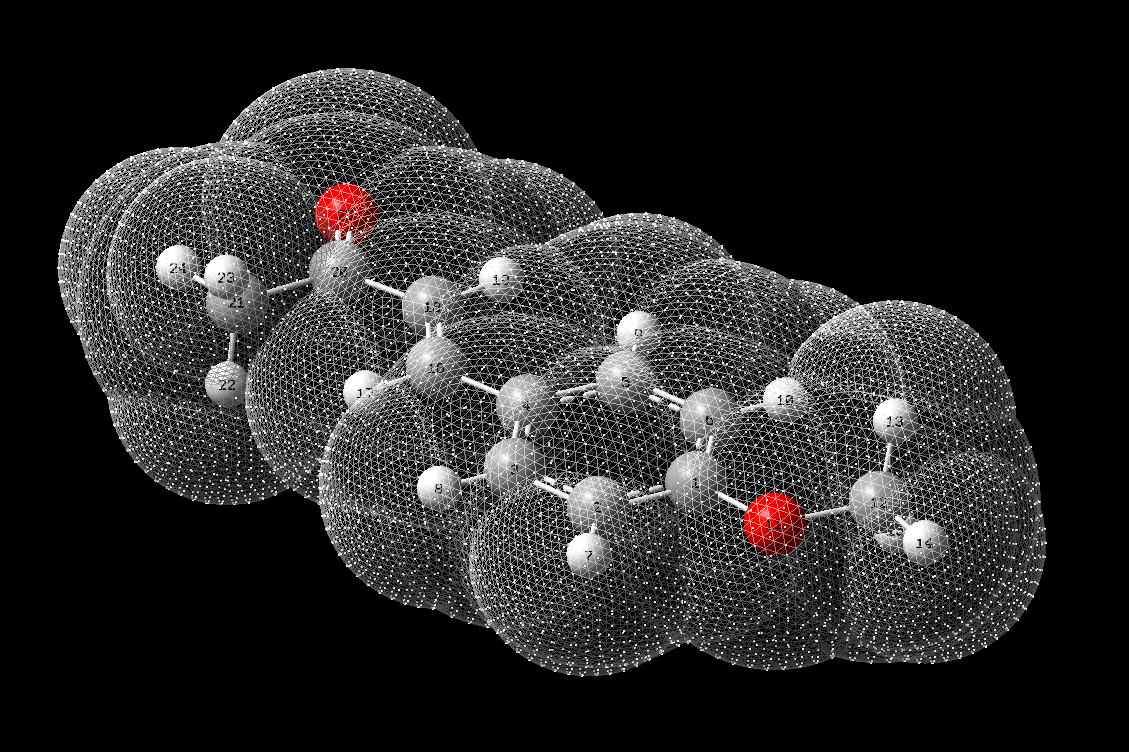
\includegraphics[width=0.85\textwidth]{images/solvation_cavity_02.png}
  \caption{A $\frac{3}{4}^{th}$ view of the Solvation Cavity}
  \label{fig:sub2}
\end{subfigure}
\caption{Model: IEFPCM, Solvent: Acetone, Molecule : Anisylidene Acetone}
\label{fig:test}
\end{figure}
\end{frame}


\begin{frame}
\frametitle{Computational Method Assessment}
\begin{itemize}
\item B3LYP/6-311G in IEFPCM (acetone) provides:
  \begin{itemize}
  \item Reasonable description of electronic structure
  \item Accounts for solvent effects on charge distribution
  \item Captures π-conjugation effects on polarizability
  \end{itemize}
\item Population analysis methods (Merz-Kollman, NTO) offer:
  \begin{itemize}
  \item Insights into charge localization
  \item Visualization of electronic transitions
  \item Understanding of molecular orbitals involved in excitation
  \end{itemize}
\item Results support experimental observations of:
  \begin{itemize}
  \item Strong UV-vis absorption
  \item Solvatochromic behavior
  \item Reactivity patterns
  \end{itemize}
\end{itemize}
\end{frame}
%%%%%%%%%%%%%%%%%%%%%%%%%%%%%%%%%%%%%%%%%%%%%%%%%%%%%%%%%%%%%%%%%%%%%%%%%%%%%%%%%%%%%%%%


\section{Acknowledgement:}
% Acknowledgments
\begin{frame}{Acknowledgments}
  \begin{block}{Research Support}
    We thank the Department of Chemical Sciences for laboratory facilities and technical support during this project.
  \end{block}
  
  \begin{block}{Faculty Support}
    Special thanks to:
    \begin{itemize}
      \item Prof. Suman De Sarkar (for providing anisaldehyde) and Prof. Debashish Halder for guidance and mentorship
      \item Lab technicians (Saroj Da only) for their constant assistance and cleaning up our mess
      \item Our classmates for providing entertainment during the course of the project (by Pritam)
      \item Swapnanil Sur for helping us doing the HRMS while we were not in Campus.
      \item Sayan da(our TA) for doing the NMR of the sample
    \end{itemize}
  \end{block}
  
  \begin{center}
    \textcolor{accentcolor}{\large Contact: \{sbs22ms076, ps22ms140\}@iiserkol.ac.in}
  \end{center}
\end{frame}
%%%%%%%%%%%%%%%%%%%%%%%%%%%%%%%%%%%%%%%%%%%%%%%%%%%%%%%%%%%%%%%%%%%%%%%%%%%%%%%%%%%%%%%%
\section{Opensourcing the data:}
\begin{frame}{All Sources are Available!!!}
\begin{figure}
    \centering
    \href{https://github.com/Shuvam-Banerji-Seal/My-Notes/tree/main/CH3204}{
\includegraphics[width=0.3\linewidth]{images/mygithub_CH3204.png}}
    
    \caption{Scan the Code or Click on it to see all the Project data and information}
    \label{fig:github}
\end{figure}
    
\end{frame}

\begin{frame}{Since we are done!}
\begin{figure}
    \centering
    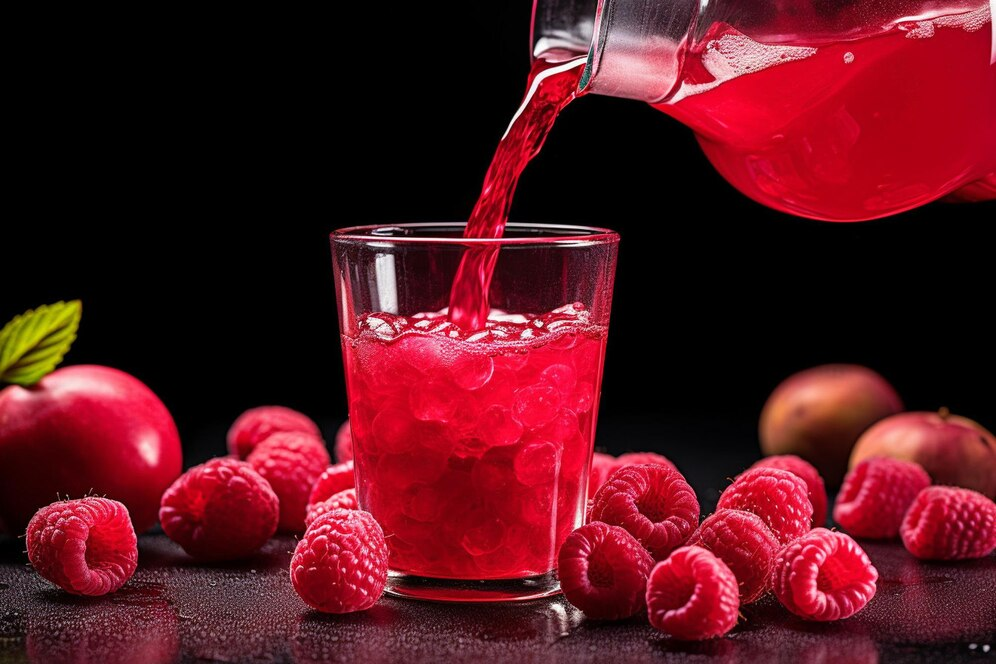
\includegraphics[width=0.5\linewidth]{images/image.png}
    \caption{Just Enjoy some Raspberry Juice}
    \label{fig:enter-label}
\end{figure}
    
\end{frame}
\begin{frame}[allowframebreaks]
\frametitle{References}
\begin{thebibliography}{14}
\setbeamertemplate{bibliography item}[text]

\bibitem[Becke, 1993]{becke1993} Becke, A. D. (1993). Density-functional thermochemistry. III. The role of exact exchange. \textit{The Journal of Chemical Physics}, 98(7), 5648--5652.

\bibitem[Besler et al., 1990]{besler1990} Besler, B. H., Merz, K. M., \& Kollman, P. A. (1990). Atomic charges derived from semiempirical methods. \textit{Journal of Computational Chemistry}, 11(4), 431--439.

\bibitem[Cancès et al., 1997]{cances1997} Cancès, E., Mennucci, B., \& Tomasi, J. (1997). A new integral equation formalism for the polarizable continuum model: Theoretical background and applications to isotropic and anisotropic dielectrics. \textit{The Journal of Chemical Physics}, 107(8), 3032--3041.

\bibitem[Frisch et al., 1984]{frisch1984} Frisch, M. J., Pople, J. A., \& Binkley, J. S. (1984). Self-consistent molecular orbital methods 25. Supplementary functions for Gaussian basis sets. \textit{The Journal of Chemical Physics}, 80(7), 3265--3269.

\bibitem[Frisch et al., 2016]{gaussian2016} Frisch, M. J., et al. (2016). Gaussian 16 Revision C.01. Gaussian Inc., Wallingford CT.

\bibitem[Krishnan et al., 1980]{krishnan1980} Krishnan, R., Binkley, J. S., Seeger, R., \& Pople, J. A. (1980). Self-consistent molecular orbital methods. XX. A basis set for correlated wave functions. \textit{The Journal of Chemical Physics}, 72(9), 650--654.

\bibitem[Lee et al., 1988]{lee1988} Lee, C., Yang, W., \& Parr, R. G. (1988). Development of the Colle-Salvetti correlation-energy formula into a functional of the electron density. \textit{Physical Review B}, 37(2), 785--789.

\bibitem[Martin, 2003]{martin2003} Martin, R. L. (2003). Natural transition orbitals. \textit{The Journal of Chemical Physics}, 118(11), 4775--4777.

\bibitem[Miertus et al., 1981]{miertus1981} Miertus, S., Scrocco, E., \& Tomasi, J. (1981). Electrostatic interaction of a solute with a continuum. A direct utilization of ab initio molecular potentials for the prevision of solvent effects. \textit{Chemical Physics}, 57(2), 117--129.

\bibitem[Mulliken, 1955a]{mulliken1955a} Mulliken, R. S. (1955). Electronic Population Analysis on LCAO-MO Molecular Wave Functions. I. \textit{The Journal of Chemical Physics}, 23(10), 1833--1840.

\bibitem[Mulliken, 1955b]{mulliken1955b} Mulliken, R. S. (1955). Electronic Population Analysis on LCAO-MO Molecular Wave Functions. II. Overlap Populations, Bond Orders, and Covalent Bond Energies. \textit{The Journal of Chemical Physics}, 23(10), 1841--1846.

\bibitem[Singh \& Kollman, 1984]{singh1984} Singh, U. C. \& Kollman, P. A. (1984). An approach to computing electrostatic charges for molecules. \textit{Journal of Computational Chemistry}, 5(2), 129--145.

\bibitem[Stephens et al., 1994]{stephens1994} Stephens, P. J., Devlin, F. J., Chabalowski, C. F., \& Frisch, M. J. (1994). Ab Initio Calculation of Vibrational Absorption and Circular Dichroism Spectra Using Density Functional Force Fields. \textit{The Journal of Physical Chemistry}, 98(45), 11623--11627.

\bibitem[Tomasi et al., 2005]{tomasi2005} Tomasi, J., Mennucci, B., \& Cammi, R. (2005). Quantum Mechanical Continuum Solvation Models. \textit{Chemical Reviews}, 105(5), 1991--2016.

\end{thebibliography}
\end{frame}
\end{document}